\documentclass[12pt,letterpaper,titlepage]{article}
\usepackage{solarized-light}
\usepackage{fontspec}
\defaultfontfeatures{Mapping=tex-text}
\usepackage{xunicode}
\usepackage{xltxtra}
\usepackage{amsmath}
\usepackage{pdfpages}
\usepackage{amsfonts}
\usepackage{amssymb}
\setcounter{secnumdepth}{0}
\usepackage{nameref}
\usepackage{enumitem}
\usepackage{environ}
\usepackage[pdf]{graphviz}
\usepackage{pdfpages}
\usepackage{pgfplots}
\usepackage{karnaugh-map}

\setmainfont{Times New Roman}
\showboxdepth=\maxdimen
\showboxbreadth=\maxdimen


\usepackage{paracol}
\usepackage{wrapfig}
\globalcounter{table}
\globalcounter{figure}
\usepackage{graphicx}
\usepackage[left=1in,right=1in,top=1in,bottom=1in]{geometry}
\graphicspath{{img/}}

\author{Jacob Abel}
\title{	Project 4
	\\\large ECE3544 CRN:82989
}

\setlength{\parskip}{0.25em}

\begin{document}
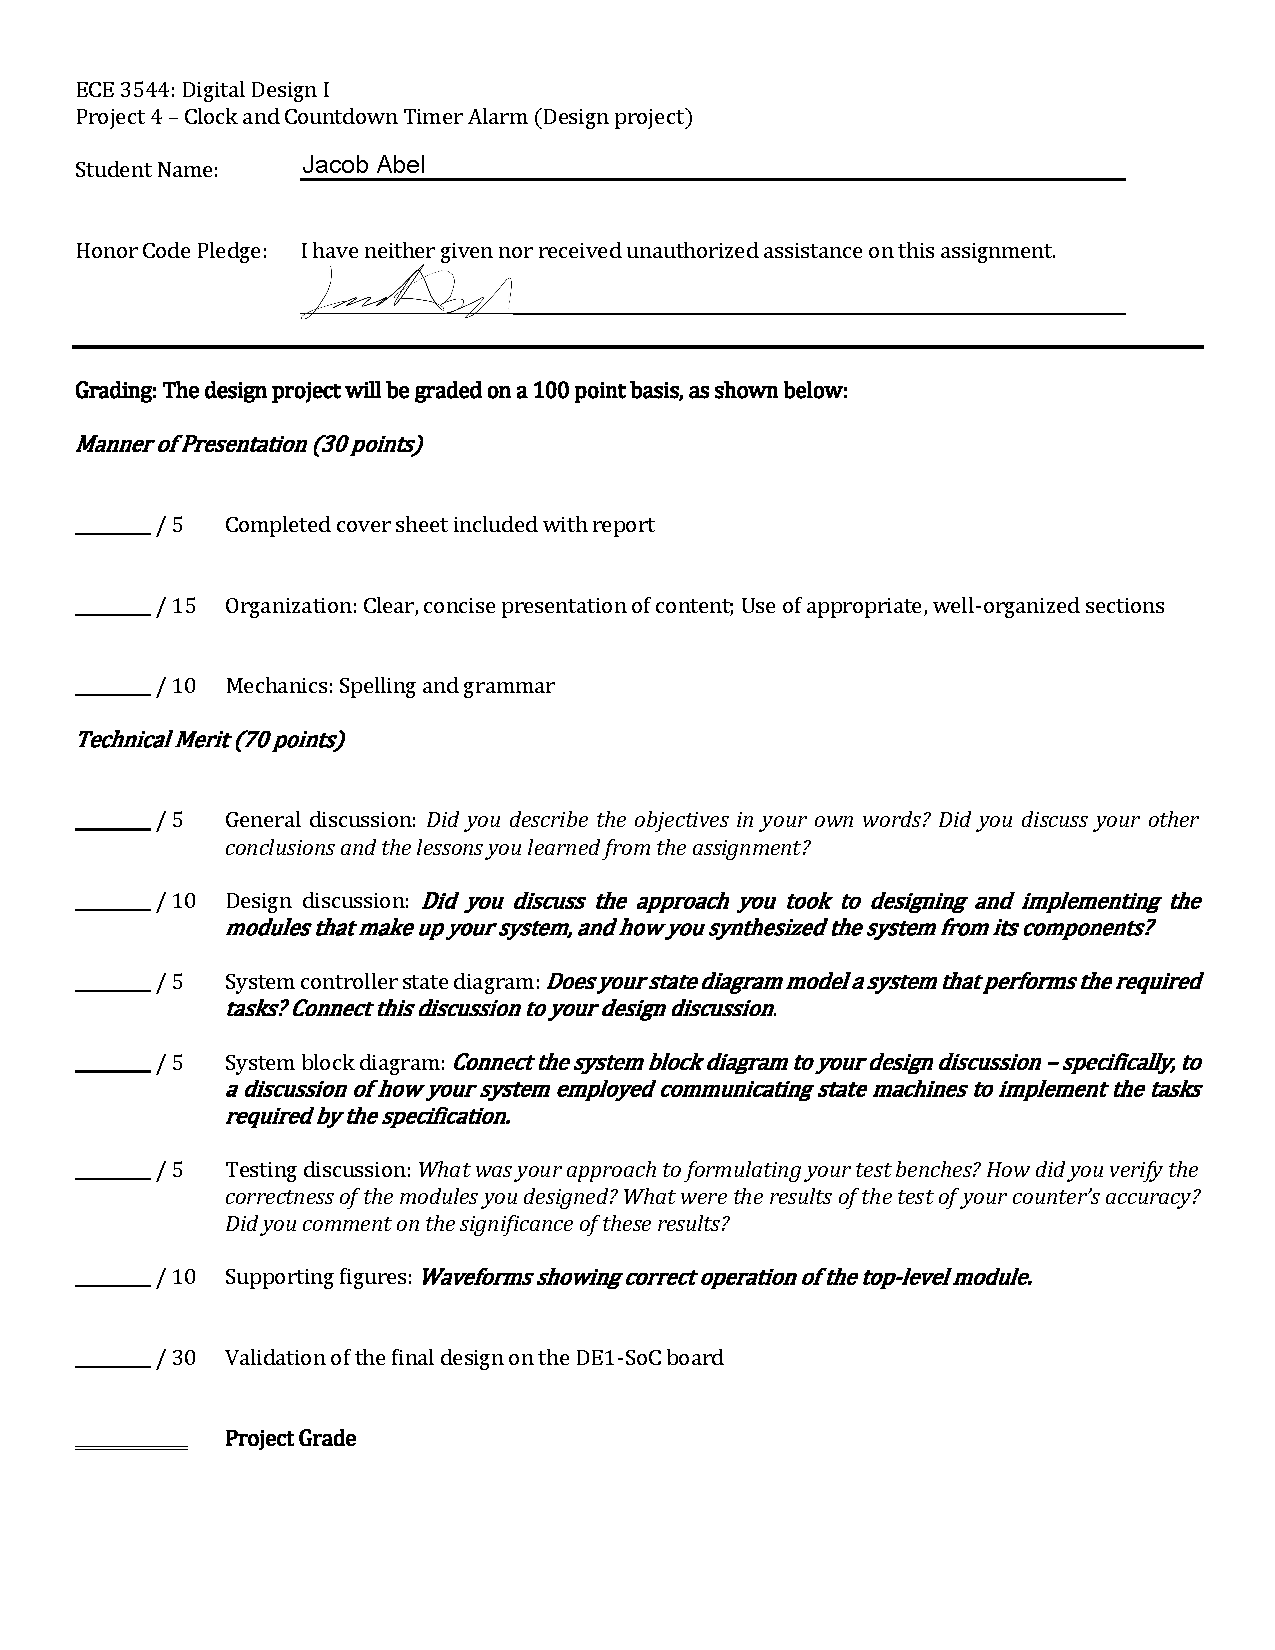
\includepdf[noautoscale]{CoverSheet.pdf}
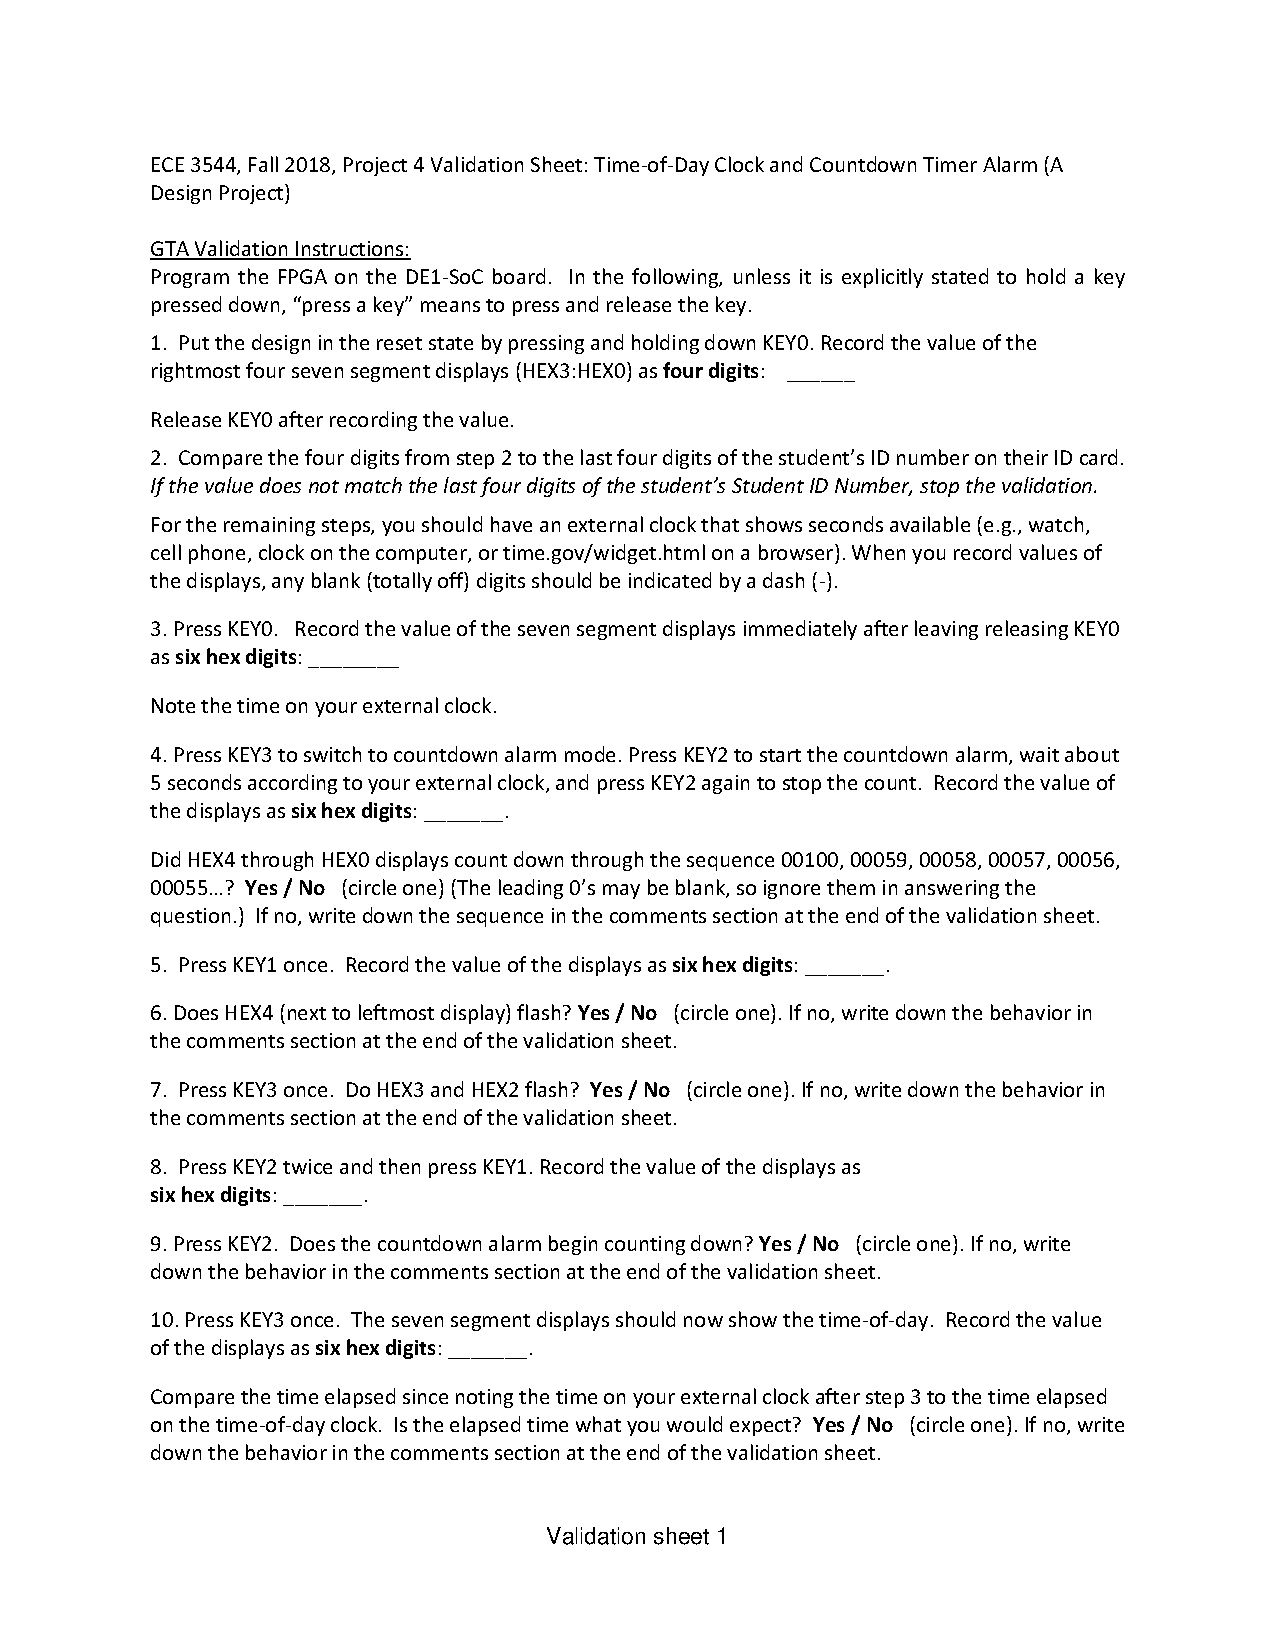
\includepdf[noautoscale]{ValidationSheet.pdf}

\maketitle
\begin{raggedright}

\section*{Objective}

\section{Primary Control FSM Diagram}

\begin{figure}[ht]
\centering
\digraph{primaryControl}{
	node [shape = plaintext] reset, alarm; 
	node [shape = ellipse];
	reset      -> INIT;
	INIT       -> CLOCKFACE;
	CLOCKFACE  -> COUNTDOWN [ label = "toggle" ];
	COUNTDOWN  -> CLOCKFACE [ label = "toggle" ];
    alarm      -> COUNTDOWN;
}
\caption{\texttt{primaryControl} Module FSM}
\end{figure}

\clearpage
\section{Countdown FSM Diagram}
\begin{figure}[ht]
\centering
\digraph{countdownsetup}{
	node [shape = plaintext] reset; 
	node [shape = ellipse];
    reset       -> DEFAULT_CDS;
	DEFAULT_CDS -> HOUR_CDS [ label = "cycle" ];
	HOUR_CDS    -> MIN_CDS [ label = "cycle" ];
	MIN_CDS     -> HOUR_CDS [ label = "cycle" ];
}
\caption{\texttt{countdown\_setup} Module FSM}
\end{figure}

\begin{figure}[ht]
\centering
\digraph{countdown}{
	node [shape = plaintext] soft_reset, hard_reset; 
	node [shape = ellipse];
    hard_reset -> DEFAULT_CD;
	soft_reset -> SETUP_CD;
    DEFAULT_CD -> SETUP_CD;
	SETUP_CD   -> START_CD [ label = "setcount" ];
    START_CD   -> WAIT_CD;
	WAIT_CD    -> RUN_CD [ label = "pause" ];
	RUN_CD     -> WAIT_CD [ label = "run" ];
	RUN_CD     -> ALARM [ label = "alarm" ];
	ALARM_CD   -> START_CD [ label = "clear" ];
}
\caption{\texttt{countdown} Module FSM}
\end{figure}
\clearpage

\section{Clockface FSM Diagram}

\begin{figure}[ht]
\centering
\digraph{clockface}{
	node [shape = plaintext] reset; 
	node [shape = ellipse];
    reset      -> DEFAULT_CF;
	DEFAULT_CF -> RUN_CF;
	RUN_CF     -> SETUP_CF [ label = "setup" ];
	SETUP_CF   -> RUN_CF [ label = "settime" ];
}
\caption{\texttt{clockface} Module FSM}
\end{figure}

\begin{figure}[ht]
\centering
\digraph{clockfacesetup}{
	node [shape = plaintext] reset; 
	node [shape = ellipse];
    reset    	-> DEFAULT_CFS;
    DEFAULT_CFS -> SEC_CFS;
	SEC_CFS  	-> MIN_CFS [ label = "cycle" ];
	MIN_CFS  	-> HOUR_CFS [ label = "cycle" ];
	HOUR_CFS 	-> SEC_CFS [ label = "cycle" ];
}
\caption{\texttt{clockface\_setup} Module FSM}
\end{figure}
\clearpage
\section{FSM Module Design}


\clearpage
\section{Project FSM Module Simulation}

\section{Conclusion}

Unfortunately while the project was very pleasant to attempt, due to scheduling issues the final deliverable is largely non functional.

\end{raggedright}
\end{document}
